\chapter{Results and Analysis} \label{ch:results-analysis}

use MCC \cite{mcc-original-paper}
\section{Sample visual output}
\subsection{The confusion matrix}
\section{A Source of ``False Negatives'' in the NCS data set} \label{sec:NCS-dataset-issues}

Sometimes the output doesn't agree with the trace, i.e. ``the ground truth'' is not 100\% correct.
sometimes either there's a false negative (reported) but something just wasn't traced in the original  1602443.

\begin{figure} \centering
	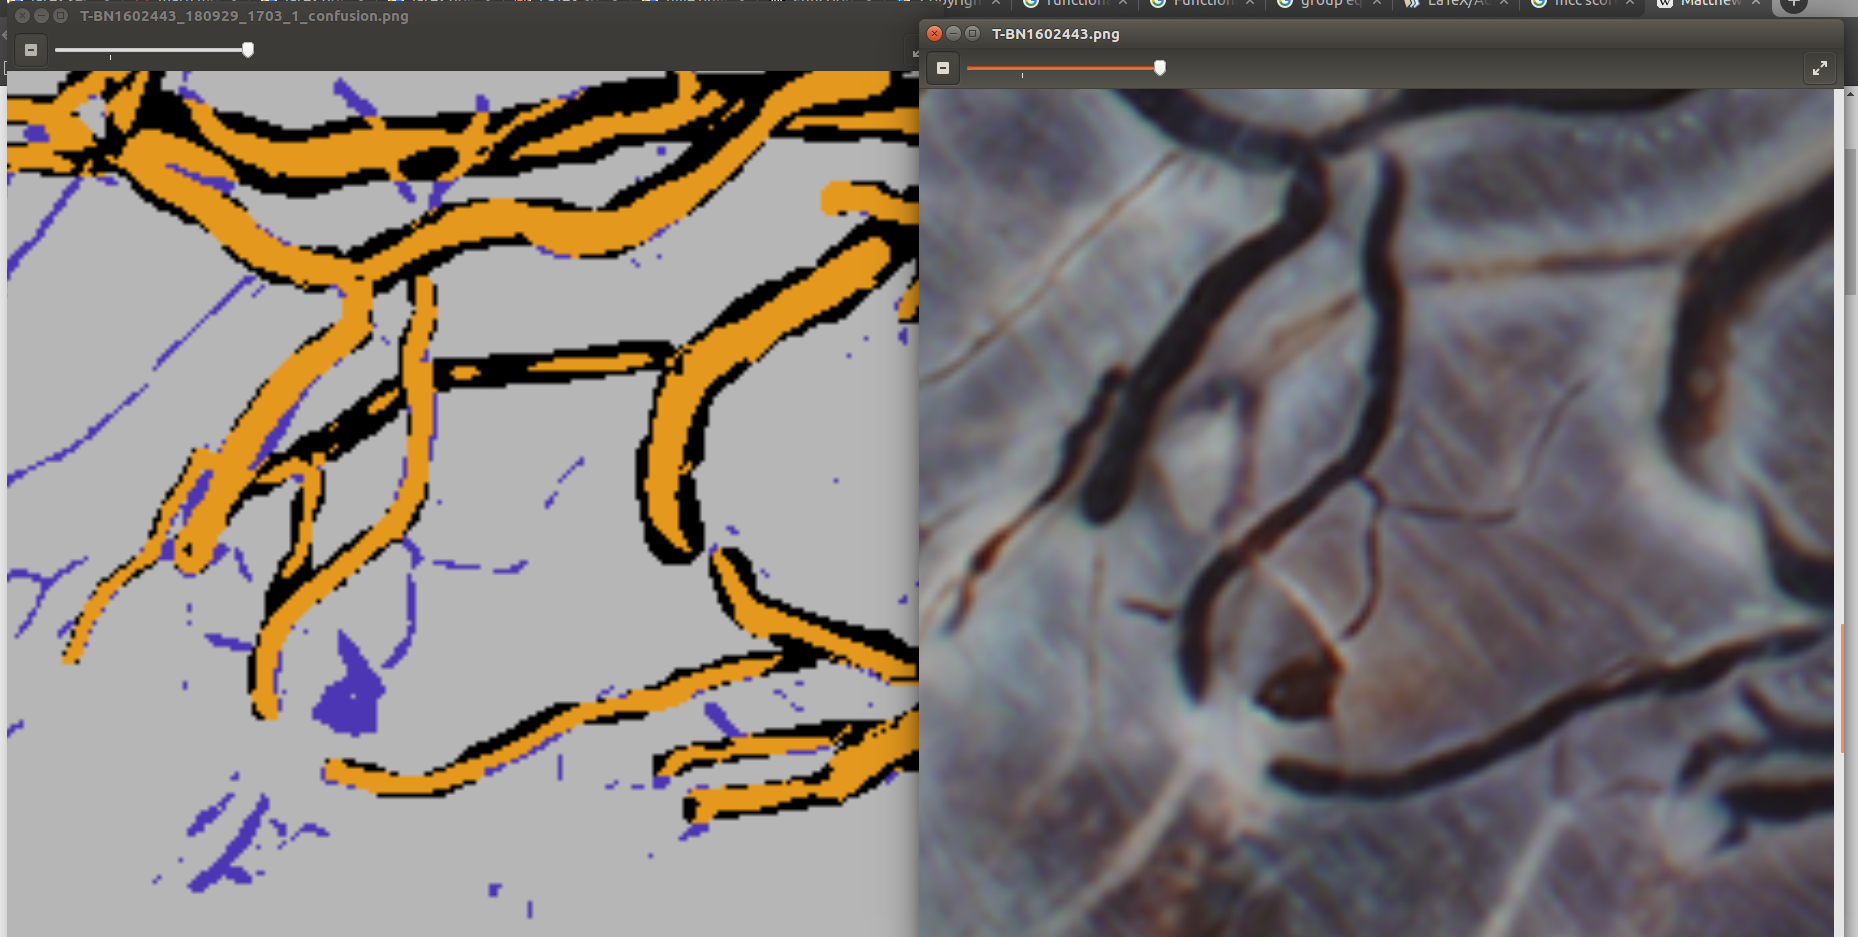
\includegraphics[width=0.8\textwidth]{kinds_of_false_positives}
	\caption{''True'' false positives and ``False'' false positives}
\end{figure}

\section{Variations in the Data Set and Imperfections of the Ground Truth}

\begin{enumerate}
\item Collar is stupid and should really be considered like a error in marking the perimeter. Throw these away or edit. Maybe make a section called discarded samples that's stupid but yeah.
\item Vessels suck sometimes. In the portion above, 1602443, there's a random blood clot which gets identified at large $\sigma$. But also the small forked shaped thing which is obviouslly a vessel doesn't get defined.
\item Too much blood (not enough?? no idea) is left in the vessels. leading to the weird white border around some vessels. you could identify these along with black center and combine them somehow. no idea.Also, holy shit, some of the white vessel ``sleeves'' ARE identified in the tracing, and some aren't. Find an example of this and whine about it.
\item Umbillical cord insertion point is stupid and obscures a lot. The tracer guesses but there's no real guiding principle AFAIK..
\item Small vessels aren't accounted for at all. Not sure how to coincide measurement in terms of scale space anymore, but should figure out how to cut off those values before running MCC metric.
\end{enumerate}





\section{Results}

This is a list of particular things I'd like to explore if I have time:

\begin{itemize}
	\item Relationship between traced pixelwidths vs the scale they were pulled from.
	\item Frangi behavior at max scale length and if there's anything that gets too large (related to first derivatives maybe?
	\item calculate the actual weingarten map eigenvectors (although this is
	probably gonna be very fake in a discrete sense).
	\item difference between using green channel and non-green channel.
\end{itemize}

\section{Answer Research Questions}
